\begin{figure}[h!]
	\centering
 	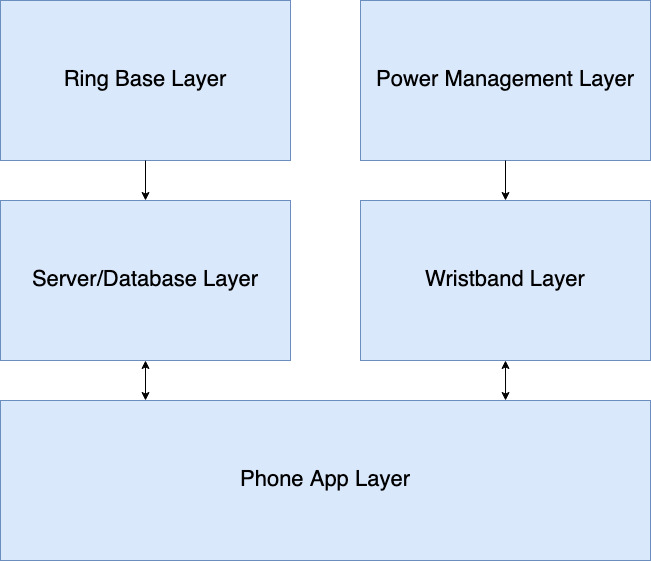
\includegraphics[width=0.60\textwidth]{images/ADS Diagrams-Basic ADS Diagram.jpg}
 \caption{A simple architectural layer diagram}
\end{figure}

\subsection{Wristband Layer Description}
This layer holds everything to do with the physical wristband. This layer includes the leds, the audio sensor, the bluetooth module, and the vibration module. This layer gets vibration commands from the Phone App layer.

\subsection{Power Management Layer Description}
This layer holds the battery, charging, and power regulation for the Wristband layer.

\subsection{Server Layer Description}
This layer holds the database of all of the user information. This layer acts as a hub between the Ring Base and Phone App and sends notifications from the Ring layer to the Phone App layer.

\subsection{Ring Base Layer}
This layer holds all of the physical sensors such as the door sensor. This layer generates notifications and alerts the Server layer.

\subsection{Phone App Layer}
This layer holds the settings for the Wristband layer and acts as an intermediary between the Server layer and the Wristband Layer.